%\setcounter{section}{0}
%\setcounter{subsection}{0}
%\setcounter{subsubsection}{0}
%\setcounter{equation}{0}
%\pagenumbering{arabic} 
%\setcounter{page}{0}    %%%%%KKD used \setcounter{page}{0}  
%\oddsidemargin 0.9 cm 
%\evensidemargin -.4 cm
%\setlength{\textwidth}{152.4 mm}
\newcommand{\pt}{ p_{T}}


\chapter{Advanced Pilup Mitigation Techniques  \label{ Advanced Pilup Mitigation Techniques}}




Grooming has been introduced in~\cite{Butterworth:2008tr} and is intended to remove soft and wide-angle radiation from the jet.  
It is typically used to reduce the overall jet mass of QCD (quark- and gluon-initiated) jets while retaining the larger jet mass for jets originating from heavy particles
such as the top quark and W/Z/H bosons.
Additionally, grooming, in the presence of pileup, can be used to reduce the dependence on pileup of jet mass.  
It should be noted that jet grooming, in general, alters the soft structure of the jet while other jet structure observables may rely on this soft structure.  

In this section, we explore the effect of grooming as a pileup mitigation method on large-R jets (R=0.8,1,2).
We consider the grooming methods: pruning~\cite{Ellis:2009me}, trimming~\cite{Krohn:2009th}, modified mass drop tagger~\cite{Dasgupta:2013ihk} and soft drop~\cite{Larkoski:2014wba}.

The pruning algorithm reclusters the constituents of the jet through the Cambridge-Aachen (CA) algorithm~\cite{Dokshitzer:1997in}, using the same distance parameter.  
At each step in the clustering algorithm, the softer of the two particles $i$ and $j$ to be merged is removed when the following conditions are met:

\begin{align}
z_{ij} & = \frac{ {\rm min}(p_{T_{i}}, p_{T_{j}})} {p_{T_{i}} + p_{T_{j}}} < z_{\rm cut} 
\label{eq:Rij1}
\end{align}

\begin{align}
\Delta R_{ij} & = \frac{2 \times r_{\rm cut} \times m_J}{p_{T}} > D_{\rm cut}
\label{eq:Rij2}
\end{align}

where $m_J$ and $\rm p_{T}$ are the mass and transverse momentum of the originally-clustered jet, and $z_{\rm cut}$ and $r_{\rm cut}$ are parameters of the algorithm.




Trimming ignores particles within a jet that fall below a dynamic threshold in $\rm p_{T}$. 
It reclusters the constituents of the jet using the kT algorithm with a radius $R_{\rm sub}$, accepting only the subjets that have $\rm p_{T_{sub}} > f_{\rm cut} \lambda_{\rm hard}$, where$ f_{\rm cut}$ is a dimensionless cutoff parameter, and $\lambda_{\rm hard}$ is some hard QCD scale chosen to equal the pT of the original jet. 






Soft-drop and modified mass drop tagger decluster the jet recursively remove soft and wide angle radiation from the jet.
The jet is reclustered using the CA algorithm.  Then the jet is declustered and at each step, subjets $j_1$ and $j_2$ are defined and the following condition is defined:

%\begin{align}
%\frac{{\rm min}(\pt_{j1},\pt_{j2})}{\pt_{j1}+\pt_{j2}} > z_{\rm cut} \times \left( \frac{\Delta R_{12}}{R_0} \right)^{\beta}
%\end{align}


where the algorithm parameters are $z_{\rm cut}$ and $\beta$.
If the condition is met, the declustering continues, otherwise only the leading $\rm p_{T}$ subjet is kept.
In the case when $\beta=0$, soft drop can be considered a generalization of the modified mass drop tagger.  

The (groomed) masses are corrected for pileup using a four-vector safe subtraction~\cite{Cacciari:2014jta}.
In the cases of soft drop, modified mass drop tagger, and trimming, the four-vector subtraction corrects the jet pT and mass at each step in the algorithm.
For pruning, the correction is applied to the final product using the pruned jet area. 
The parameters for the grooming algorithms explored in this study are summarized in Table~\ref{tab:groom}.



 
\begin{table}[h]
\begin{center}
\begin{tabular}{|c|c|}
    \hline
    grooming algorithm & parameter(s) \\
    \hline
    \hline    
    {Pruning} & $z_{\rm cut}$ = 0.1, $r_{\rm cut}$ = 0.5\\
    & $z_{\rm cut}$ = 0.05, $r_{\rm cut}$ = 0.5\\
    & $z_{\rm cut}$ = 0.1, $r_{\rm cut}$ = 0.75\\
    & $z_{\rm cut}$ = 0.05, $r_{\rm cut}$ = 0.75\\        
    \hline
    {Trimming} & $r_{\rm sub}$ = 0.2, $pT_{\rm frac}$ = 0.05\\
    & $r_{\rm sub}$ = 0.2, $pT_{\rm frac}$ = 0.03\\    
    & $r_{\rm sub}$ = 0.1, $pT_{\rm frac}$ = 0.03\\    
    & $r_{\rm sub}$ = 0.3, $pT_{\rm frac}$ = 0.03\\            
    \hline
    {Soft drop/MMDT} & $z_{\rm cut}$ = 0.1,$\beta$  = -1 \\
     & $z_{\rm cut}$ = 0.1,$\beta$  = 0 \\    
     & $z_{\rm cut}$ = 0.1,$\beta$  = 1 \\    
     & $z_{\rm cut}$ = 0.1,$\beta$  = 2 \\              
    \hline    
\end{tabular}
\caption{Summary of grooming parameters}
\label{tab:groom}
\end{center}
\end{table}



\subsection{Simulation-only results at high pileup}


The performance of various groomers is evaluated at higher pileup scenarios which expected in LHC Run II.
For a given $\rm p_{T}$ bin, we evaluate the jet mass resolution for both background QCD jets and signal W jets.  
In the signal case, the jet mass resolution is evaluated after matching the jet to the W boson direction at the particle level.  
In the background case, a $\Delta R$ matching is done between the particle level jet and the jet after full detector reconstruction where $\Delta R < 0.3$.
In each comparison, the {\it groomed} particle level jet is compared against its corresponding matched detector-level reconstructed jet.

We first evaluate the performance of groomers based on particle flow input collection with and without CHS to understand the effect.
We show the average jet mass for PF and CHS background QCD jets in Fig.~\ref{fig:grooming_PFvCHS}.
The left column shows the average jet mass as a function of pileup for jets using particle flow inputs.
The right column shows the average jet mass as a function of the pileup for jets using particle flow inputs including CHS.
We see generally that the CHS jet masses are more stable against pileup.  
The trimming algorithm is generally stable against pileup regardless of input while the pruning algorithm shows the most pileup dependence, particularly using particle flow inputs.
The soft drop algorithm has a mild pileup dependence.


\begin{figure}[h!]
\centering
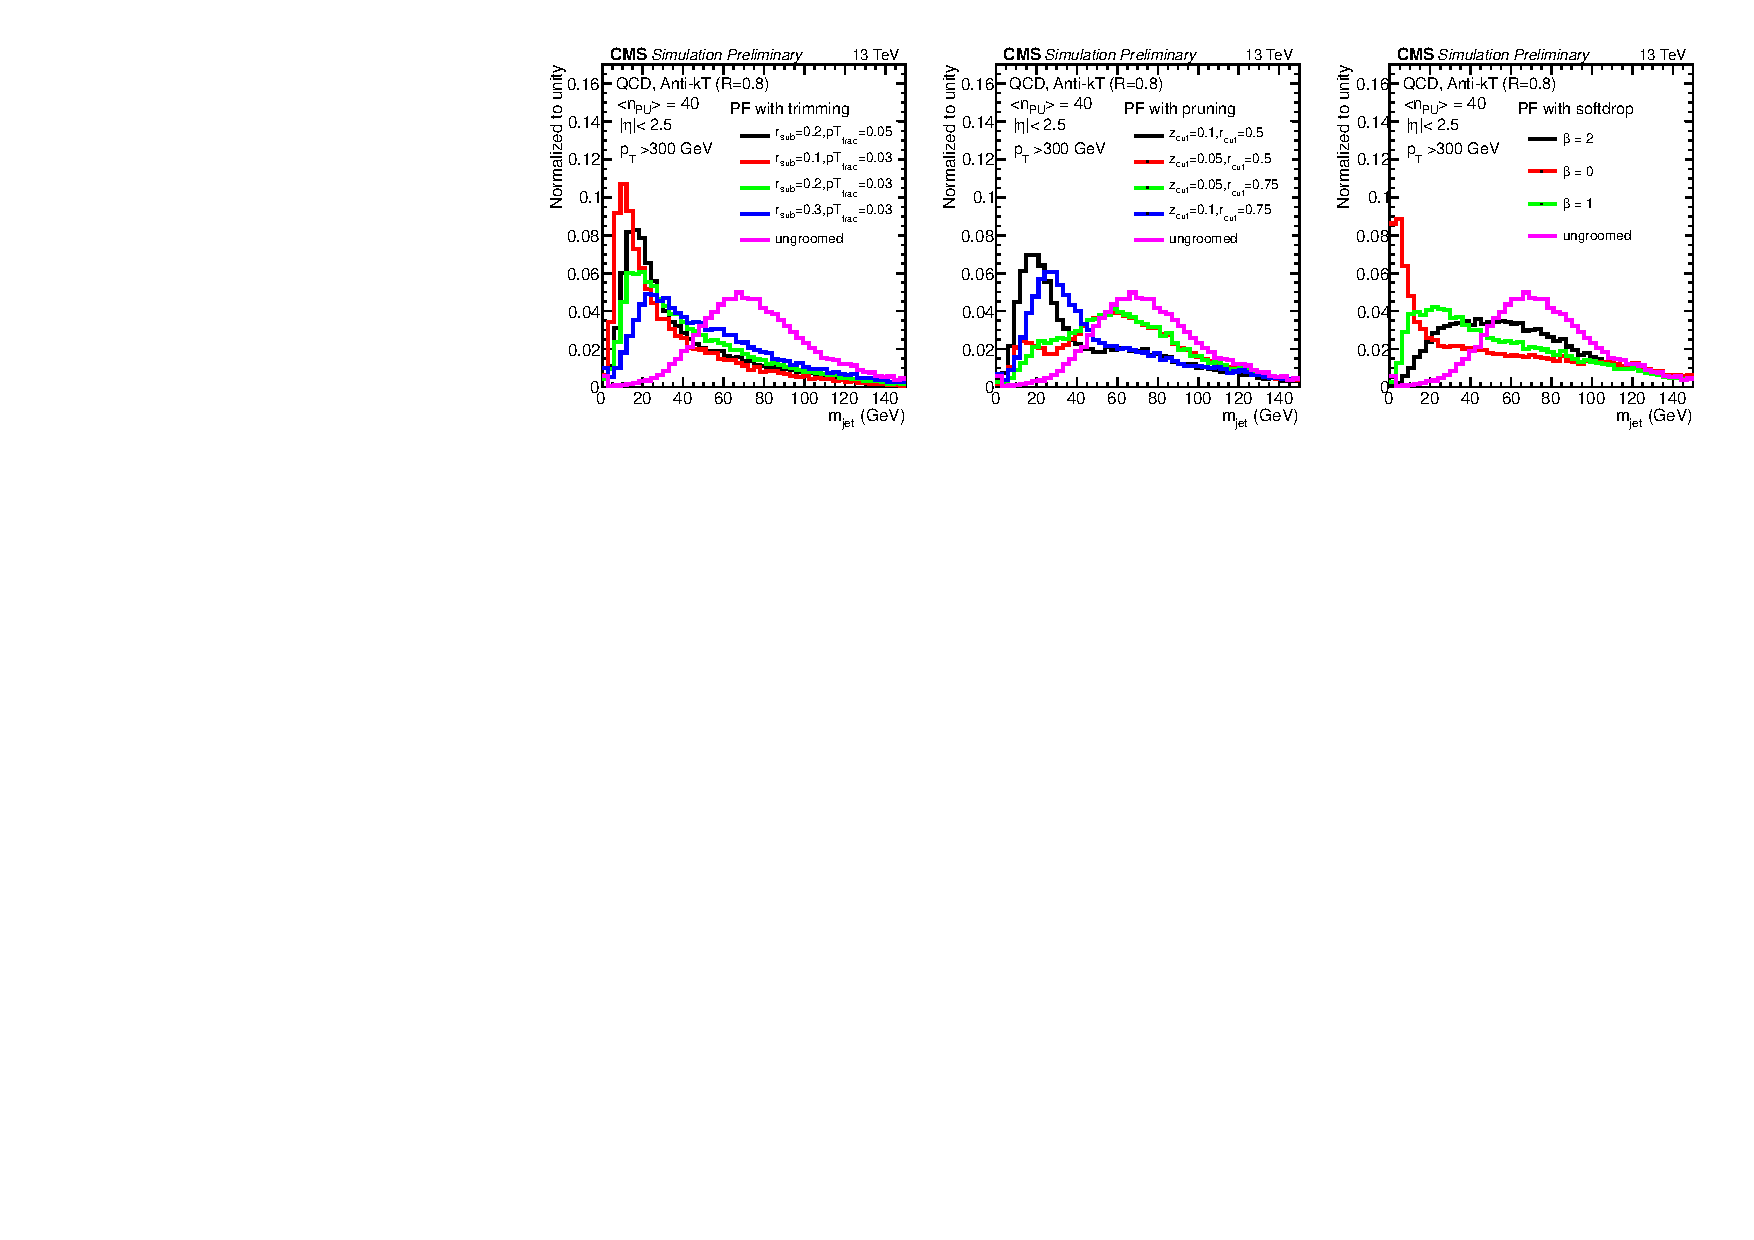
\includegraphics[width=1.00\textwidth]{/home/bibhu/Desktop/PhDThesis/PhDThesis/chapter8/1DPF_QCD.pdf}
\caption{Jet mass distribution for PF  QCD jets for different groming parameters. The PF jets are safe subtracted.}
\label{fig:jet_mass_pf_all_groomer}
\end{figure}


\begin{figure}[h!]
\centering
%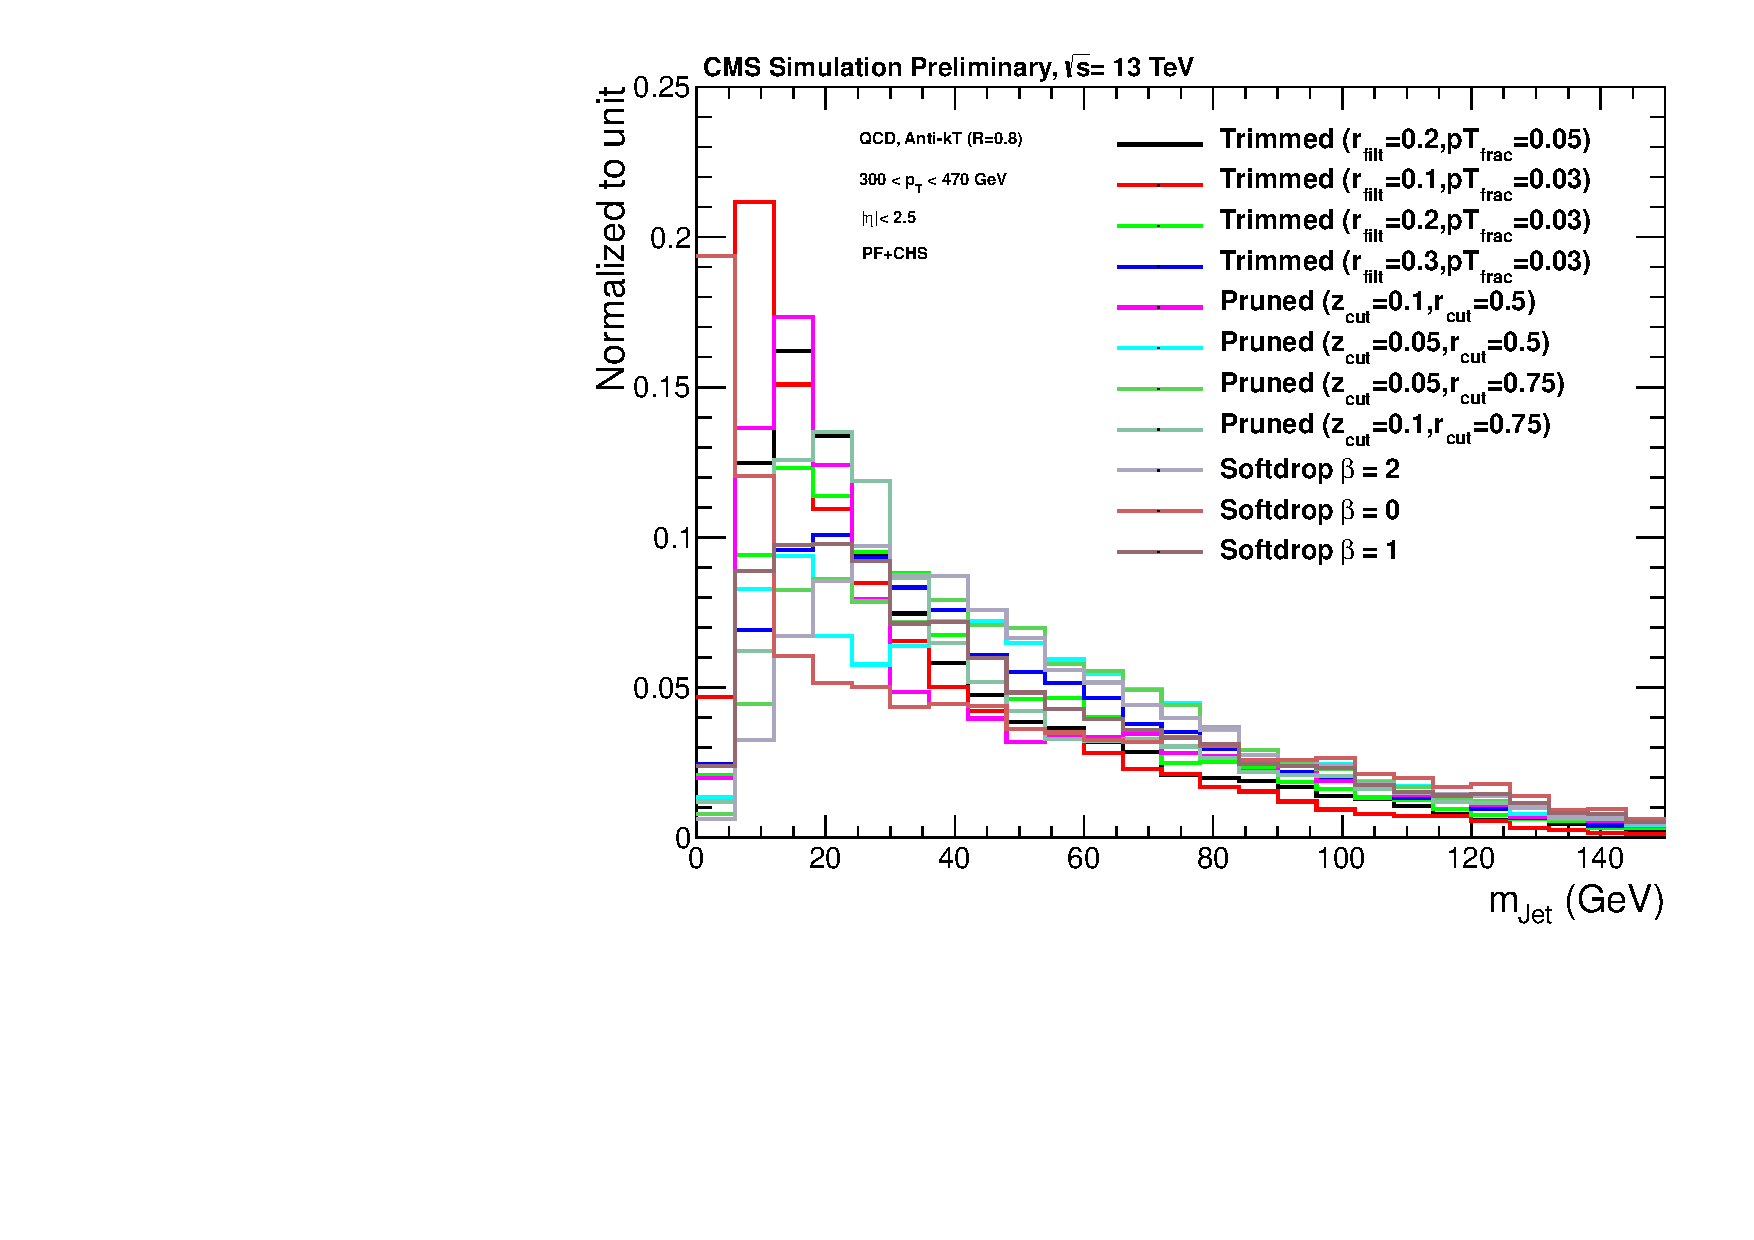
\includegraphics[width=0.60\textwidth]{Figures/puMit/Bibhu/QCD_all_groomer.pdf}
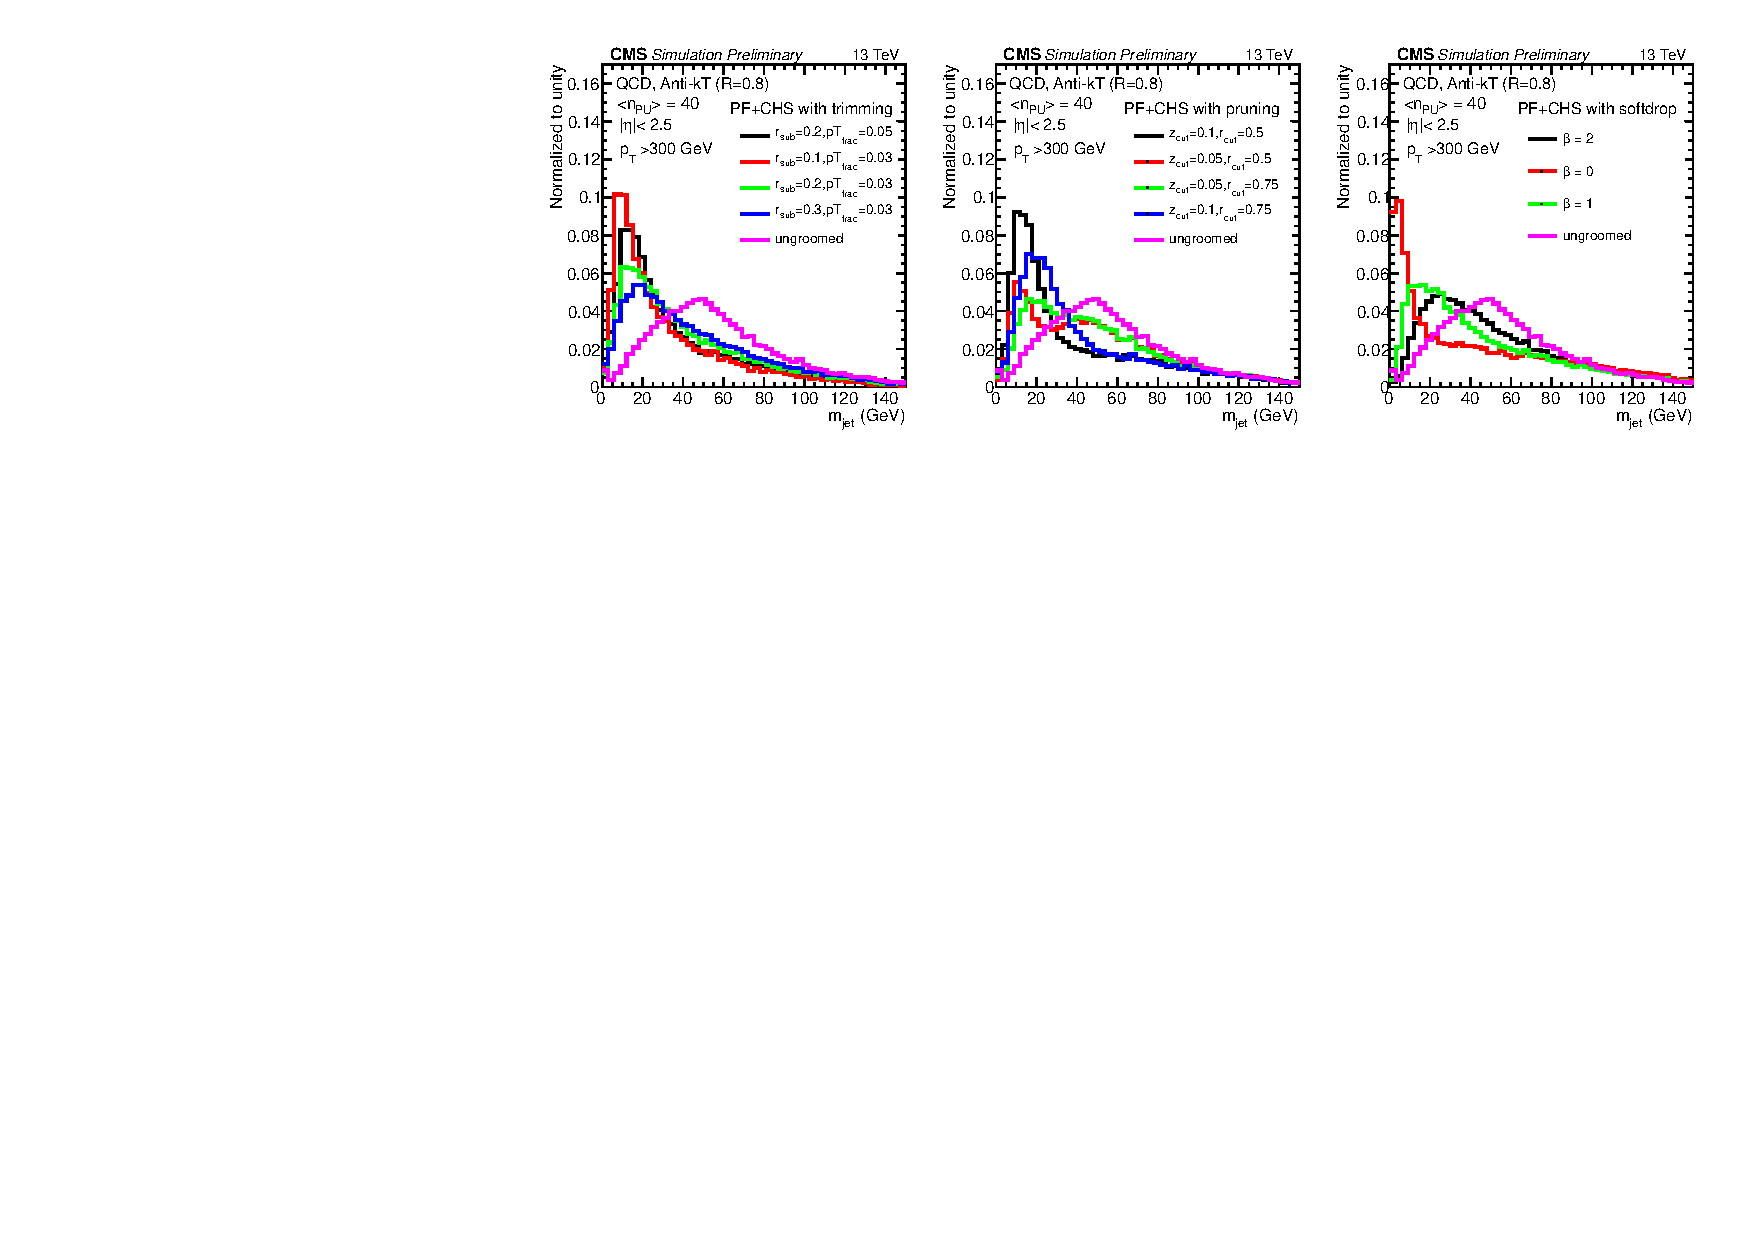
\includegraphics[width=1.00\textwidth]{/home/bibhu/Desktop/PhDThesis/PhDThesis/chapter8/1DPFCHS_QCD.pdf}
\caption{Jet mass distribution for PF+CHS  QCD jets for different groming parameters. The PFCHS jets are safe subtracted.}
\label{fig:jet_mass_chs_all_groomer}
\end{figure}



\begin{figure}[h!]
\centering
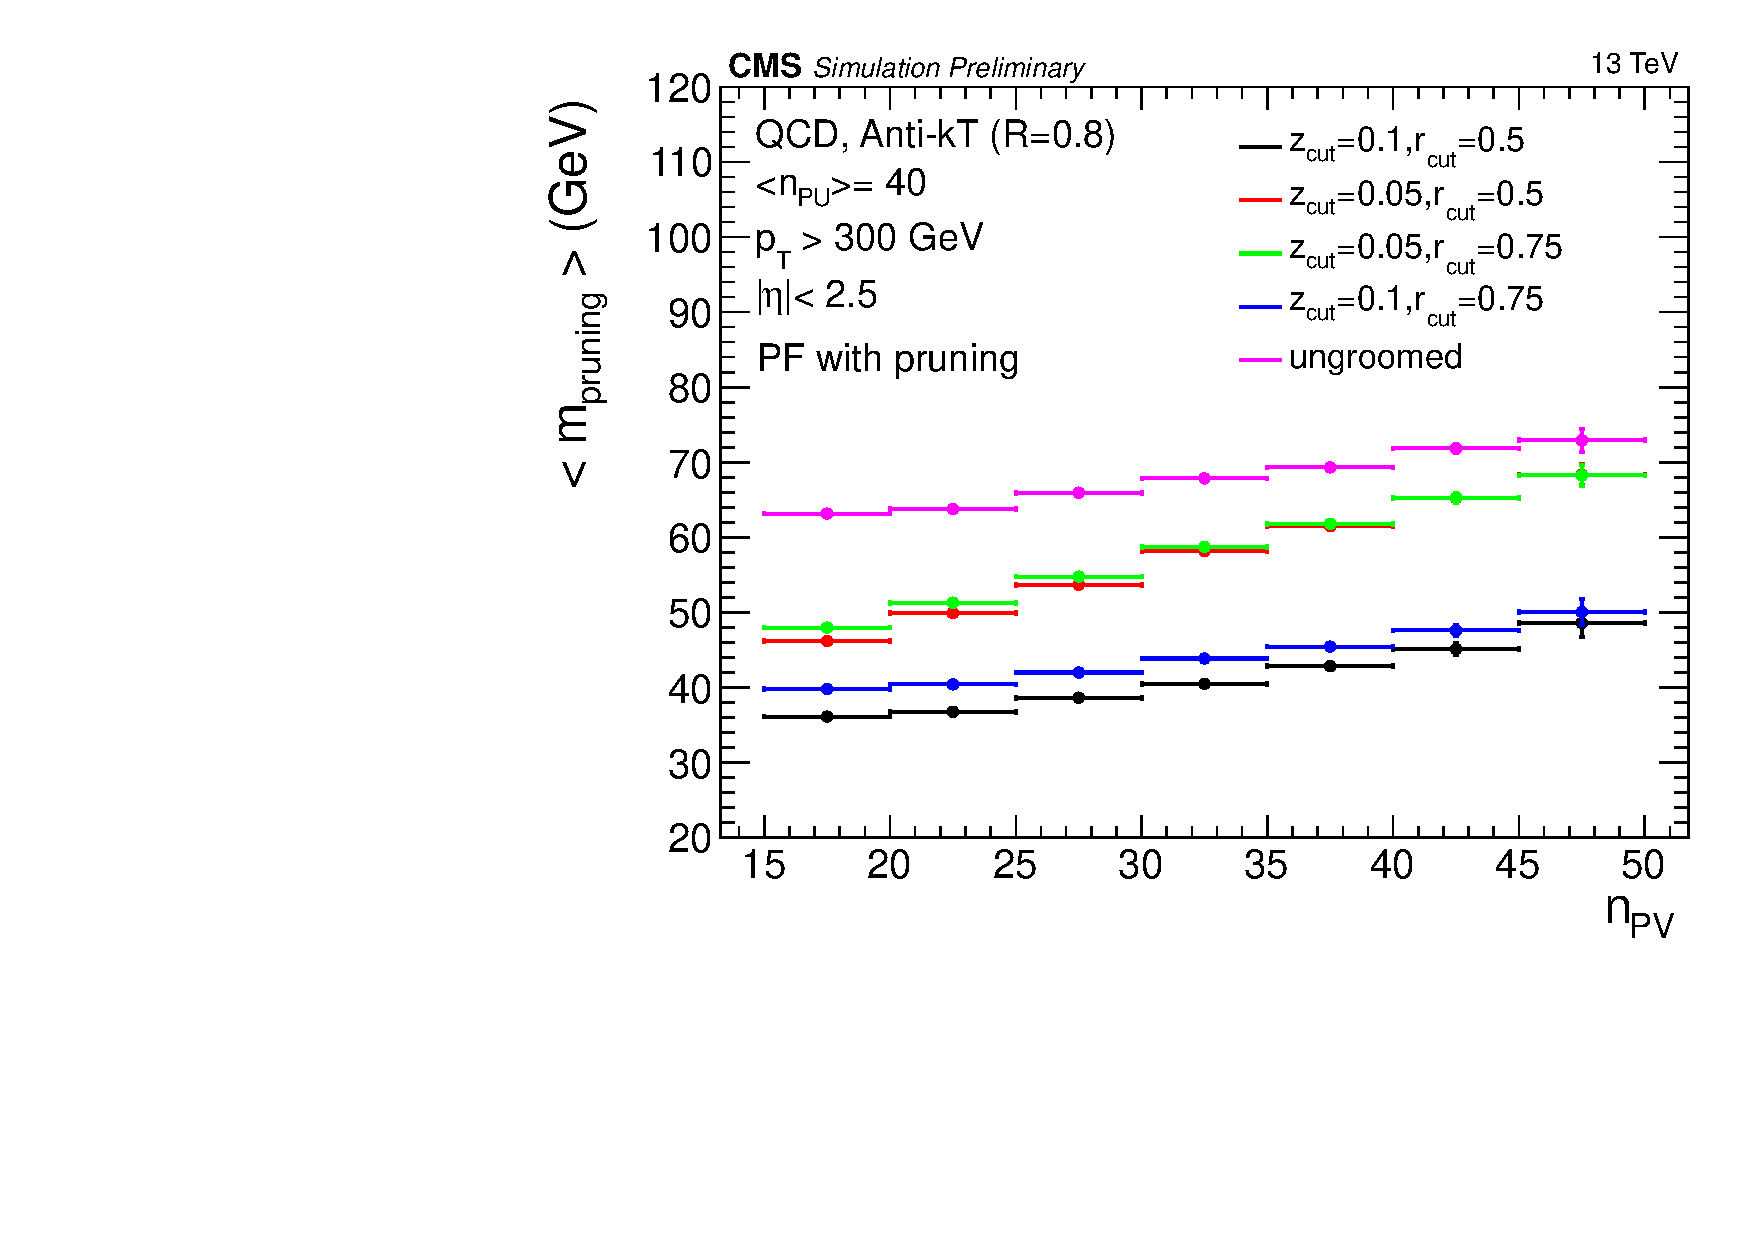
\includegraphics[width=0.47\textwidth]{/home/bibhu/Desktop/PhDThesis/PhDThesis/chapter8/AvJetmass_Vs_npv_PF_prun.pdf}
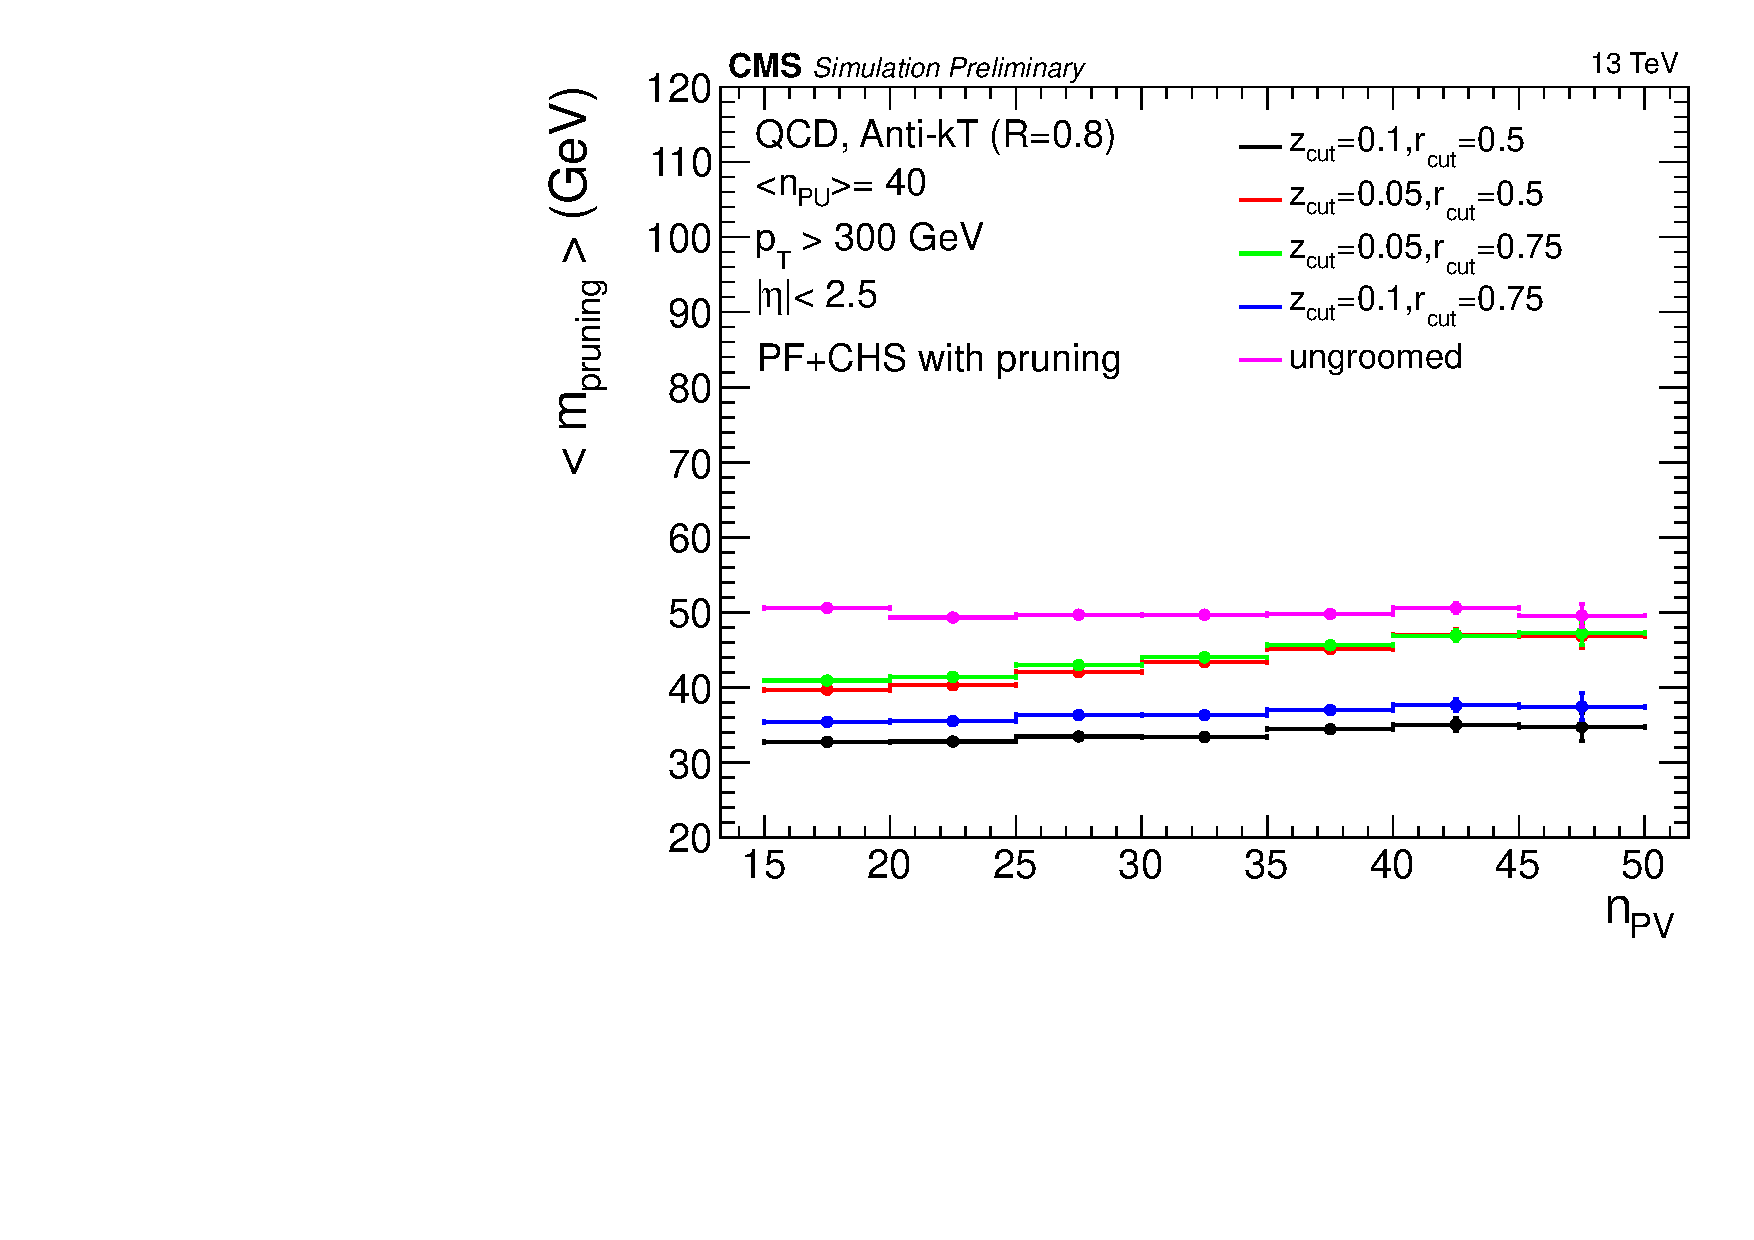
\includegraphics[width=0.47\textwidth]{/home/bibhu/Desktop/PhDThesis/PhDThesis/chapter8/AvJetmass_Vs_nPV_PFCHS_prun.pdf}\\
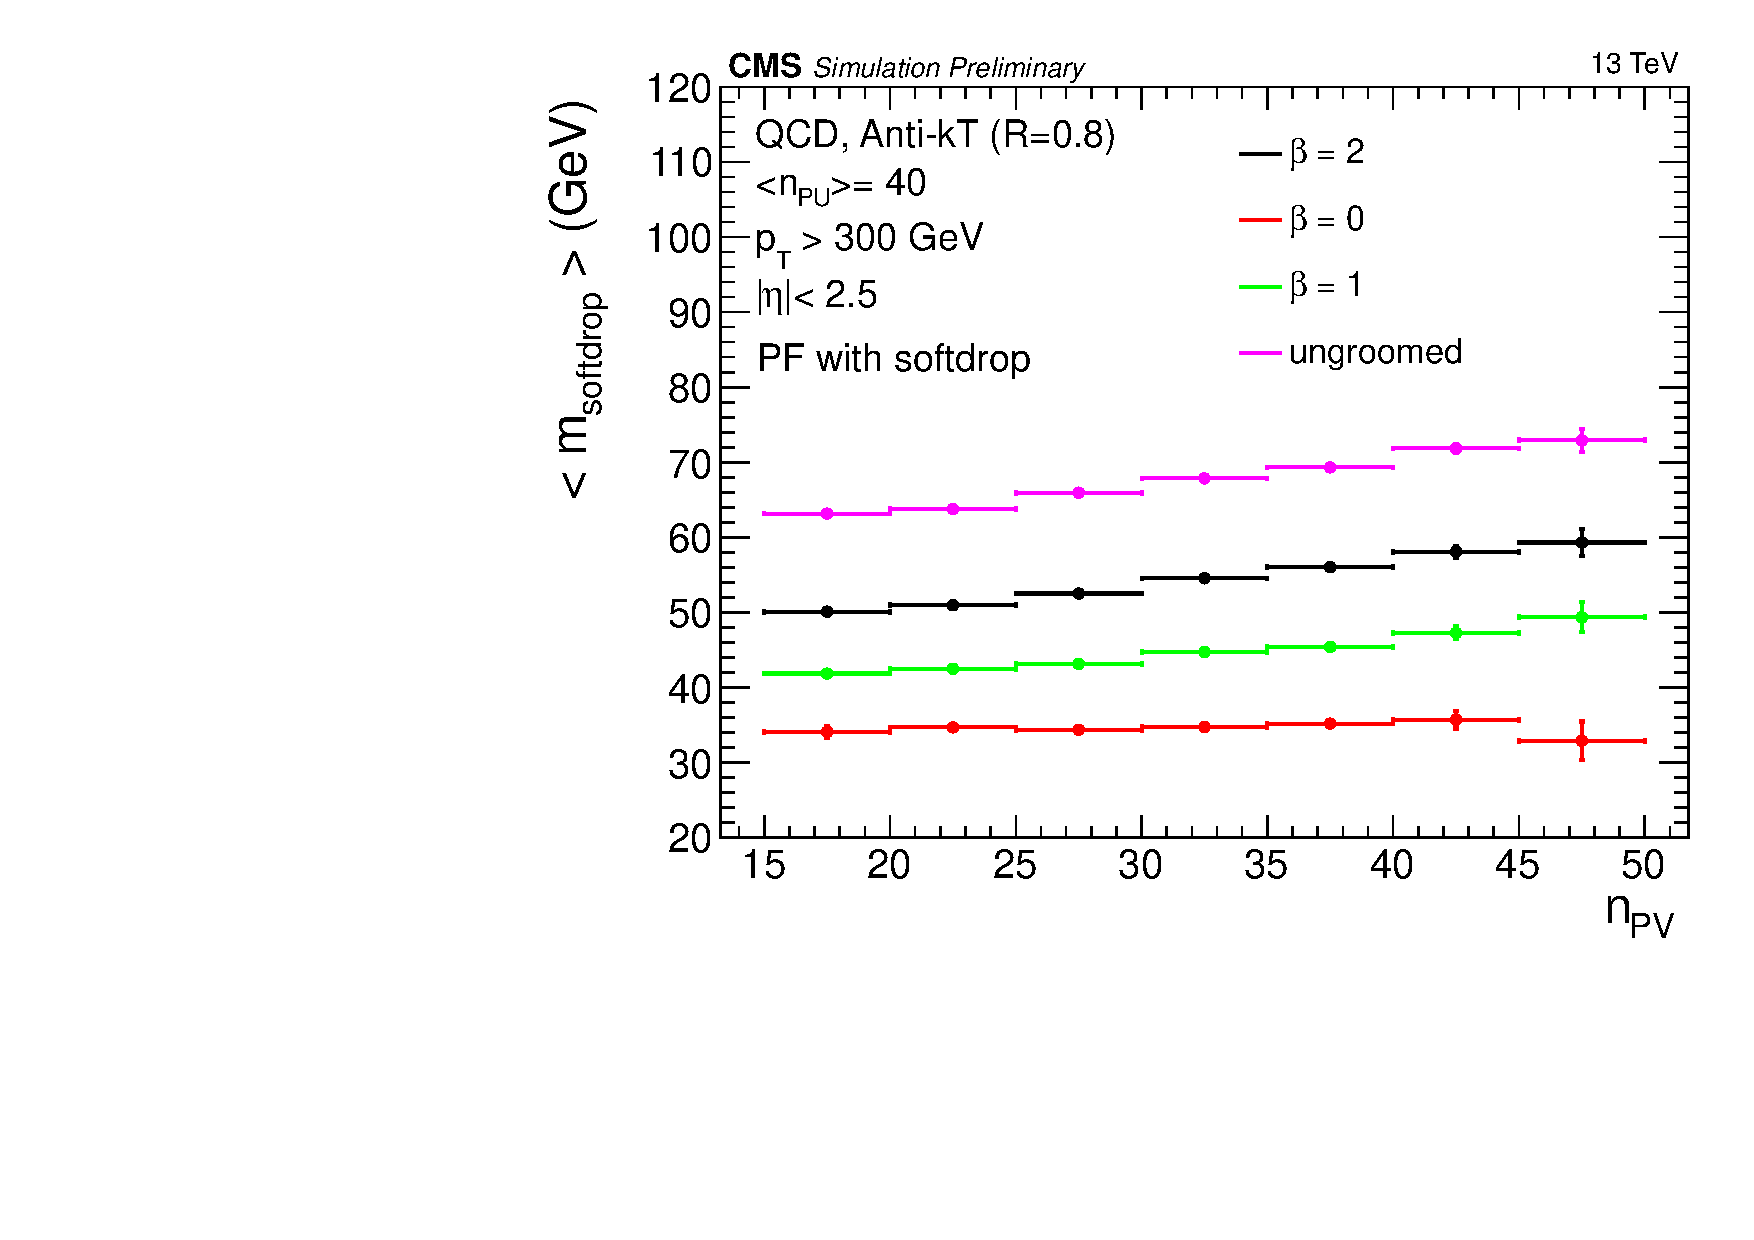
\includegraphics[width=0.47\textwidth]{/home/bibhu/Desktop/PhDThesis/PhDThesis/chapter8/AvJetmass_Vs_nPV_PF_SD.pdf}
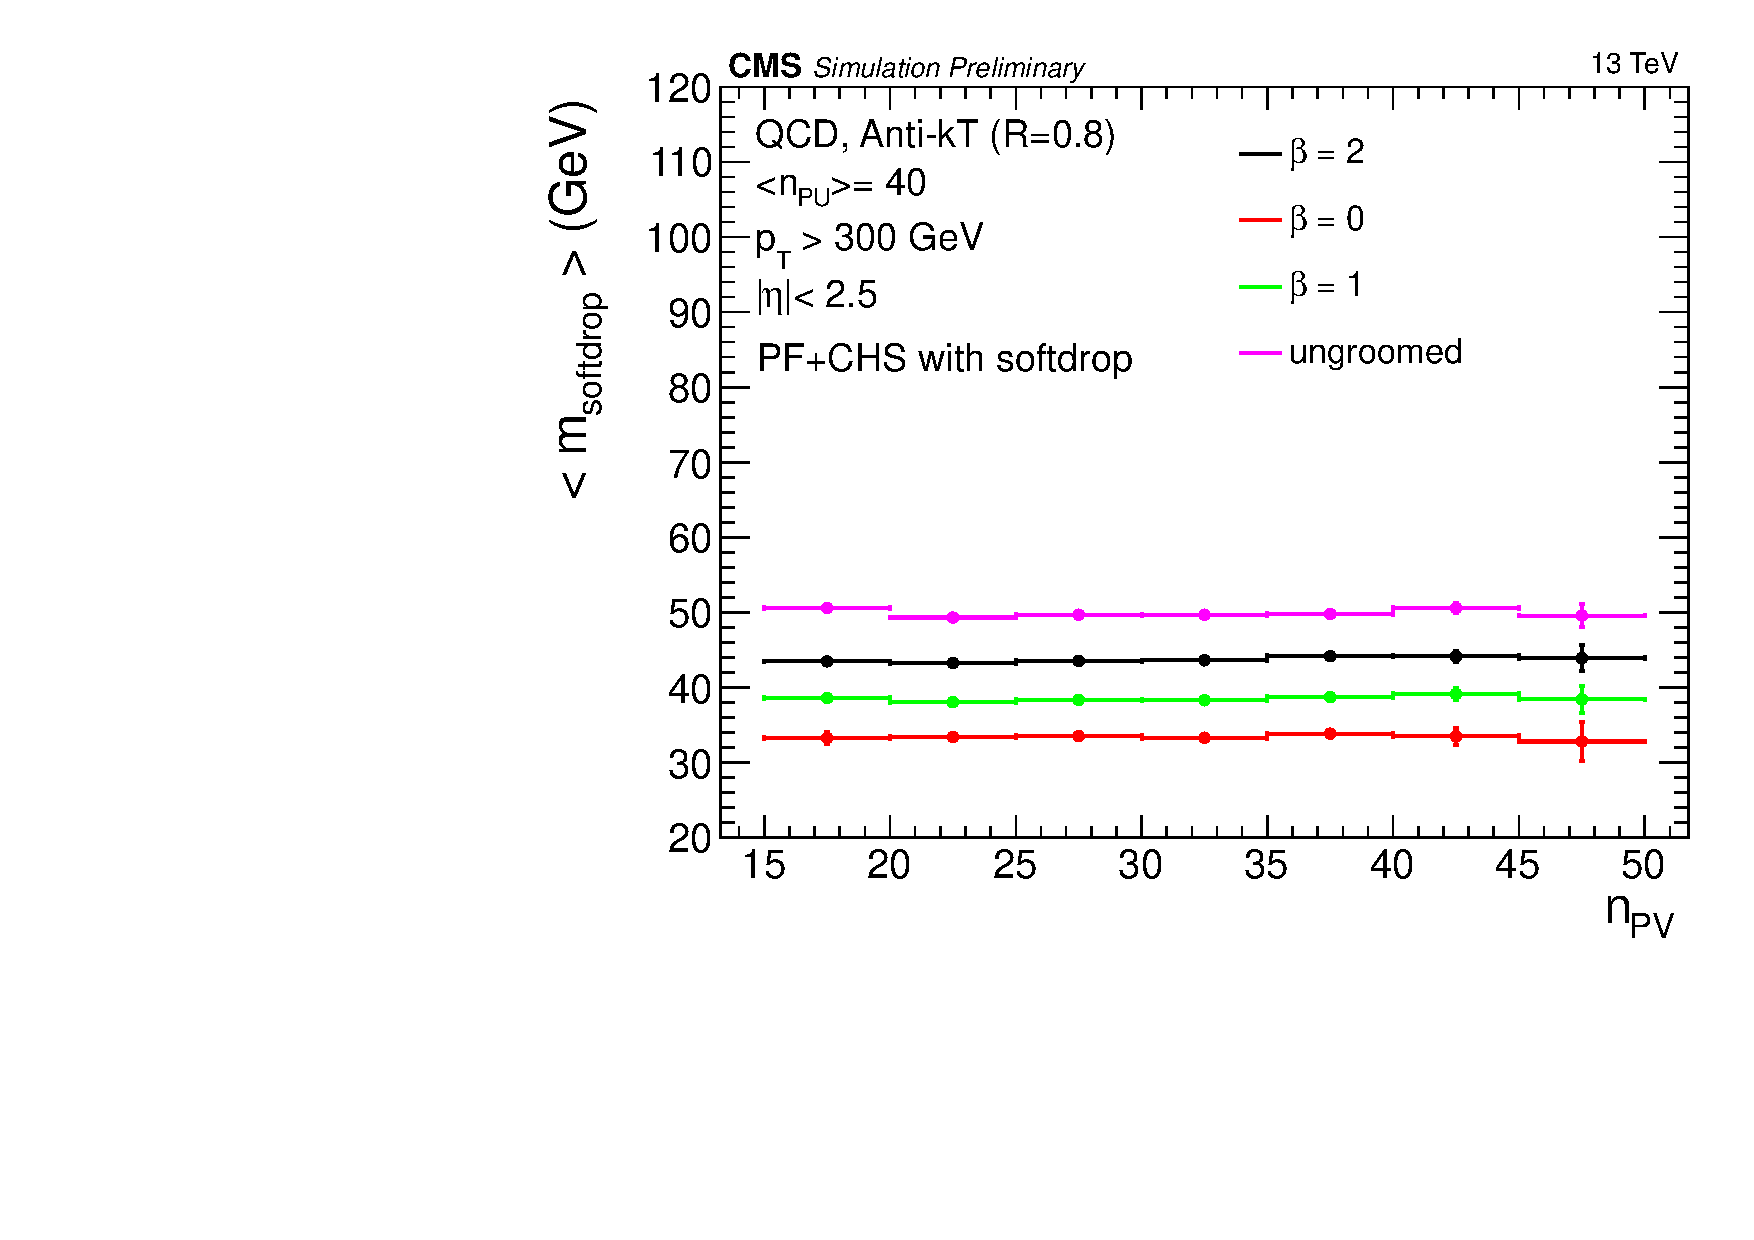
\includegraphics[width=0.47\textwidth]{/home/bibhu/Desktop/PhDThesis/PhDThesis/chapter8/AvJetmass_Vs_nPV_PFCHS_SD.pdf}\\
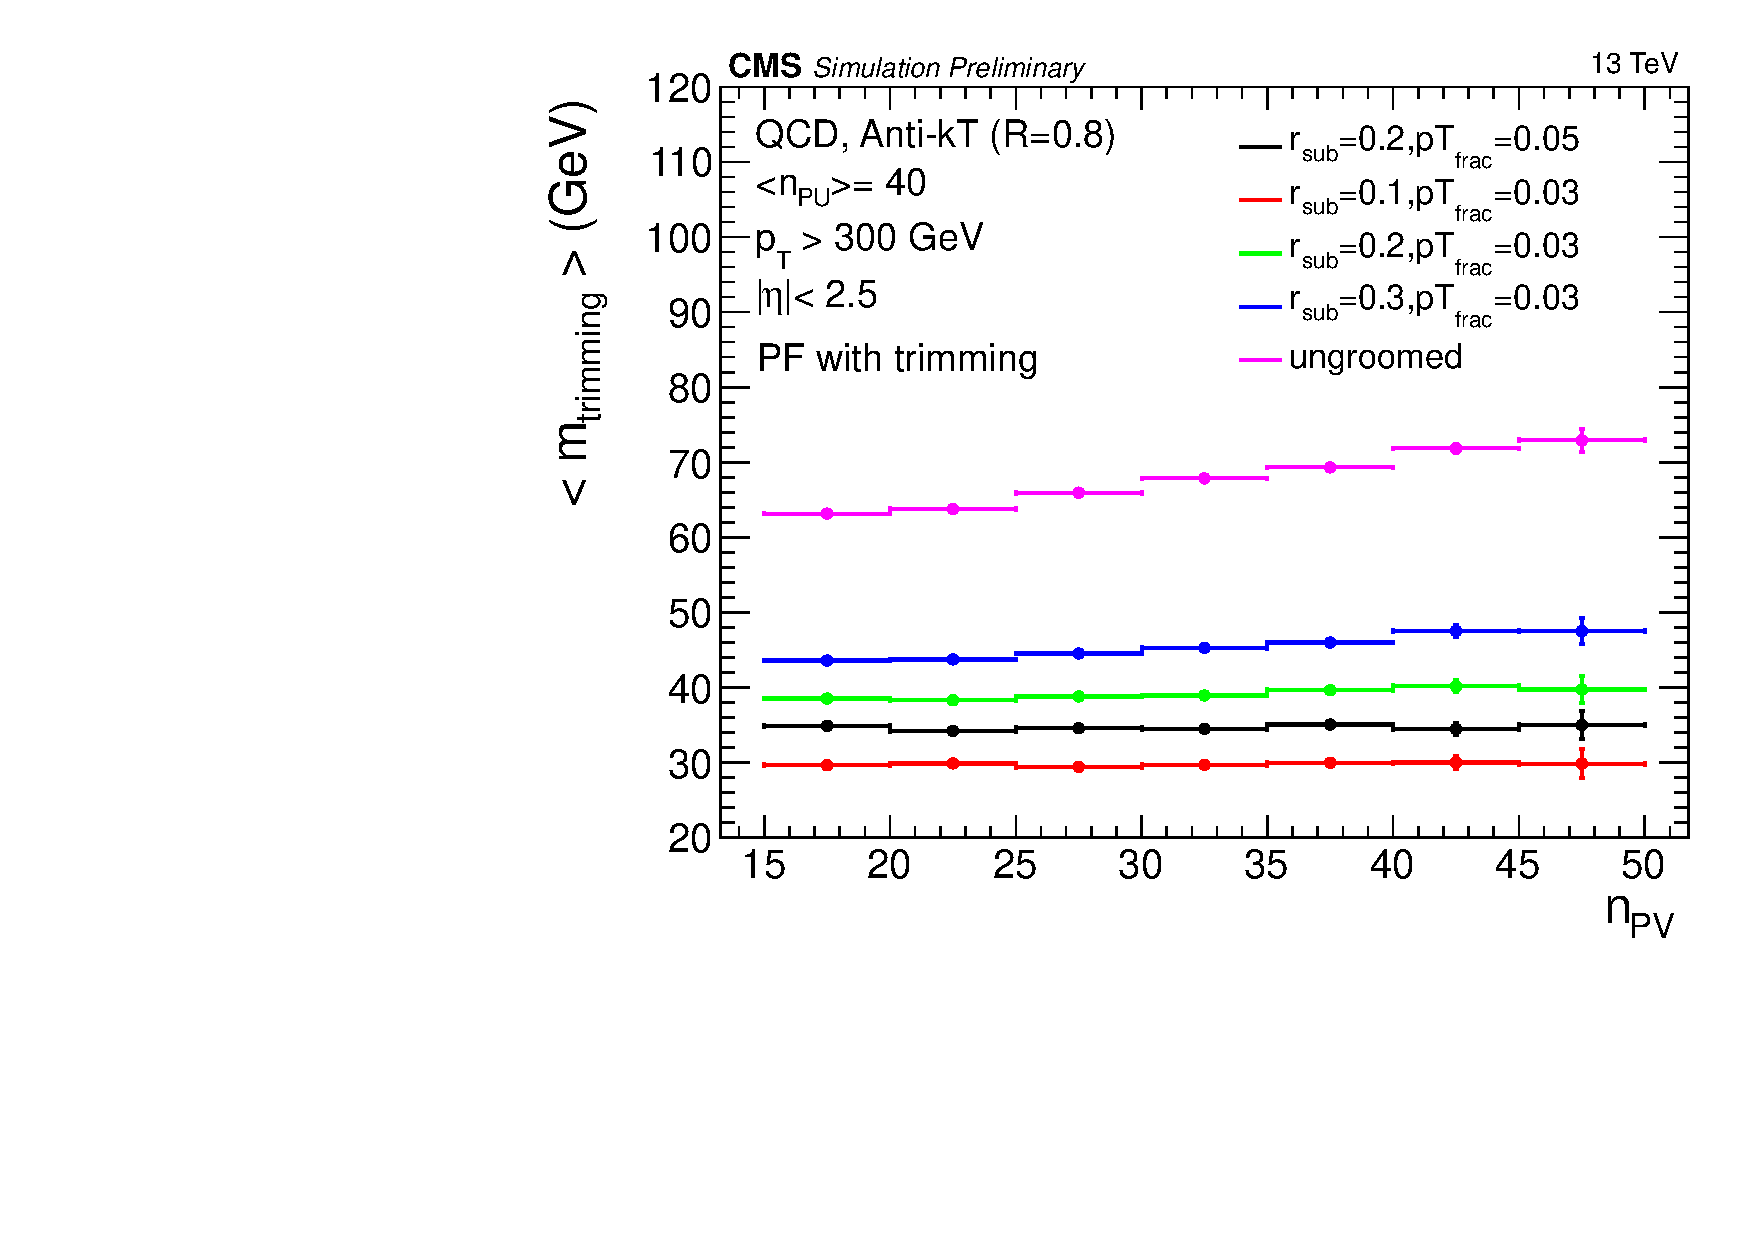
\includegraphics[width=0.47\textwidth]{/home/bibhu/Desktop/PhDThesis/PhDThesis/chapter8/AvJetmass_Vs_nPV_PF_trim.pdf}
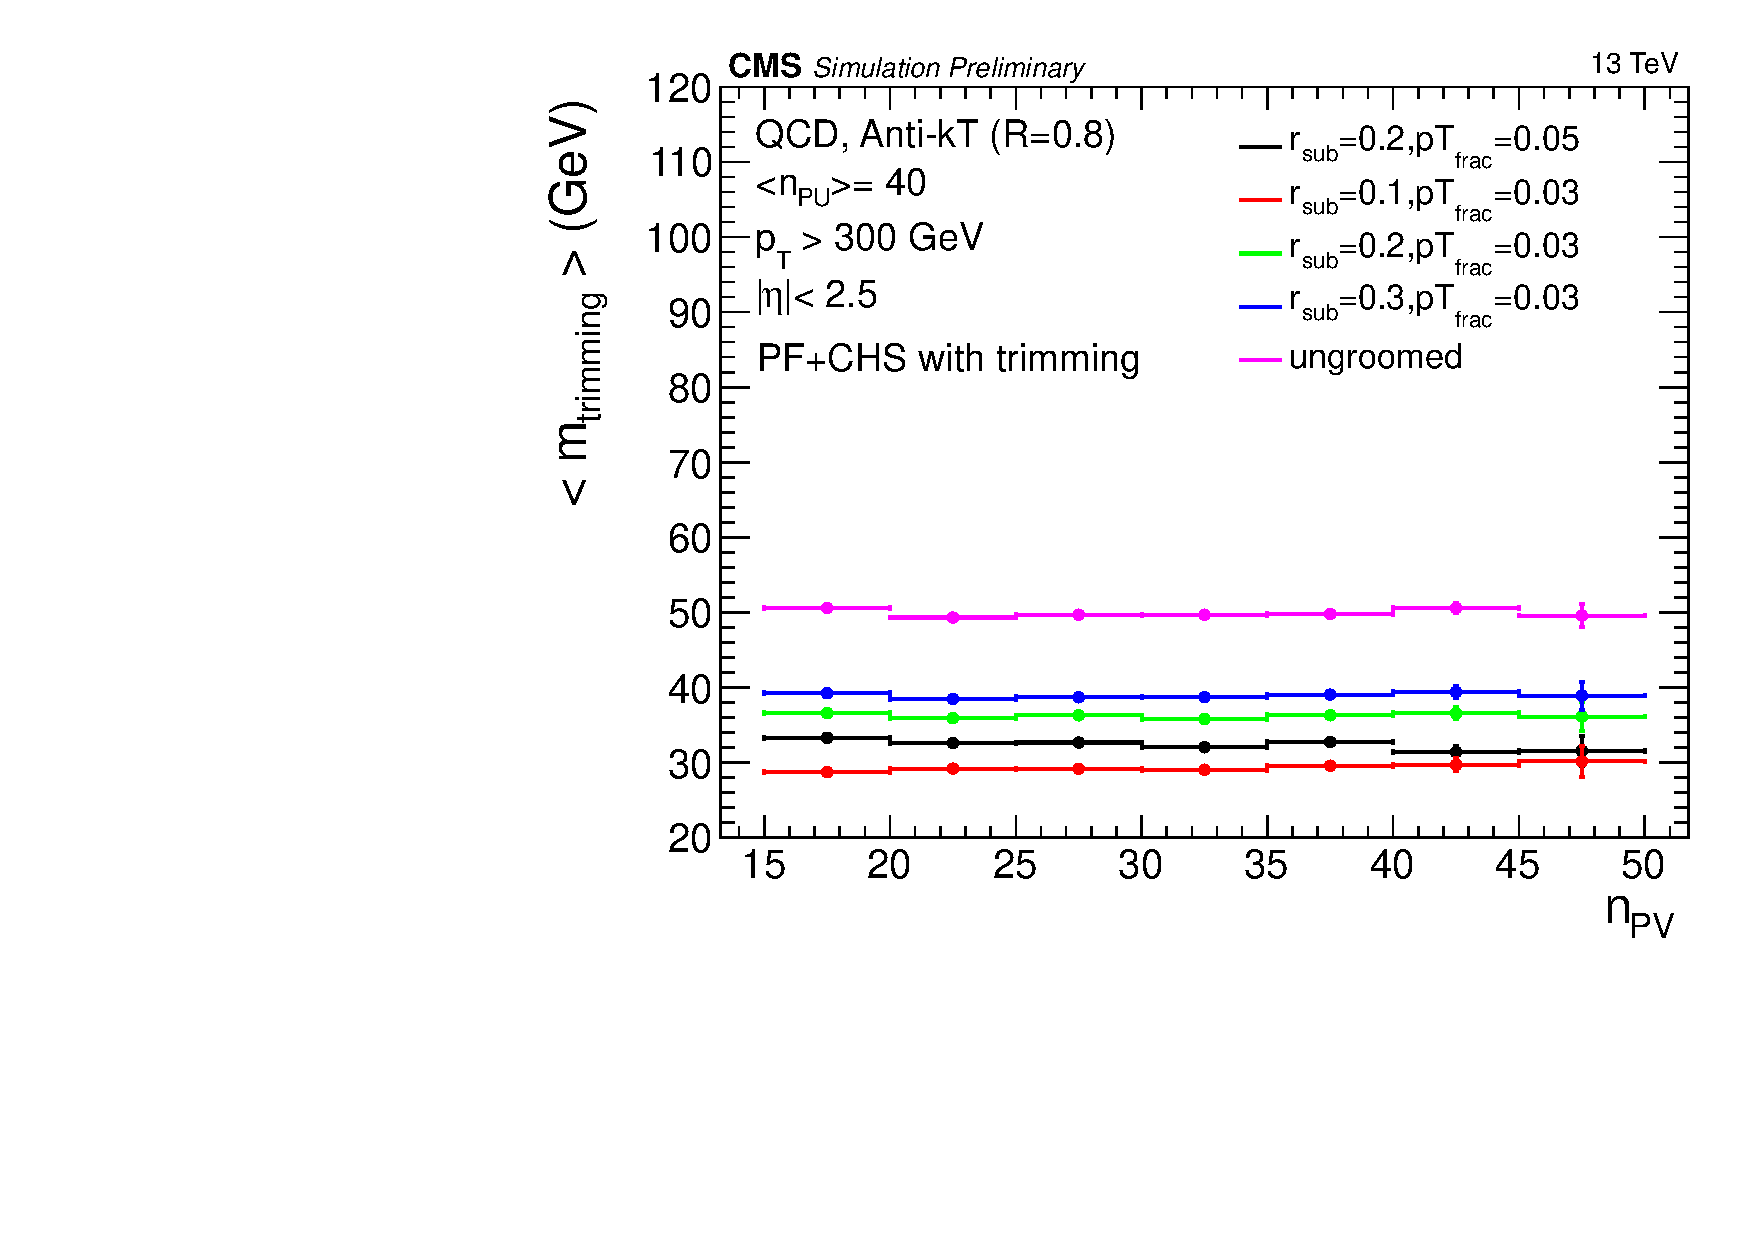
\includegraphics[width=0.47\textwidth]{/home/bibhu/Desktop/PhDThesis/PhDThesis/chapter8/AvJetmass_Vs_nPV_PFCHS_trim.pdf}\\
\caption{Pileup dependence of the average jet mass for PF jets (left) and PFCHS jets (right) for several grooming algorithms and parameters. Both PF and PFCHS jets are safe subtracted.}
\label{fig:grooming_PFvCHS}
\end{figure}






\begin{figure}[h!]
\centering
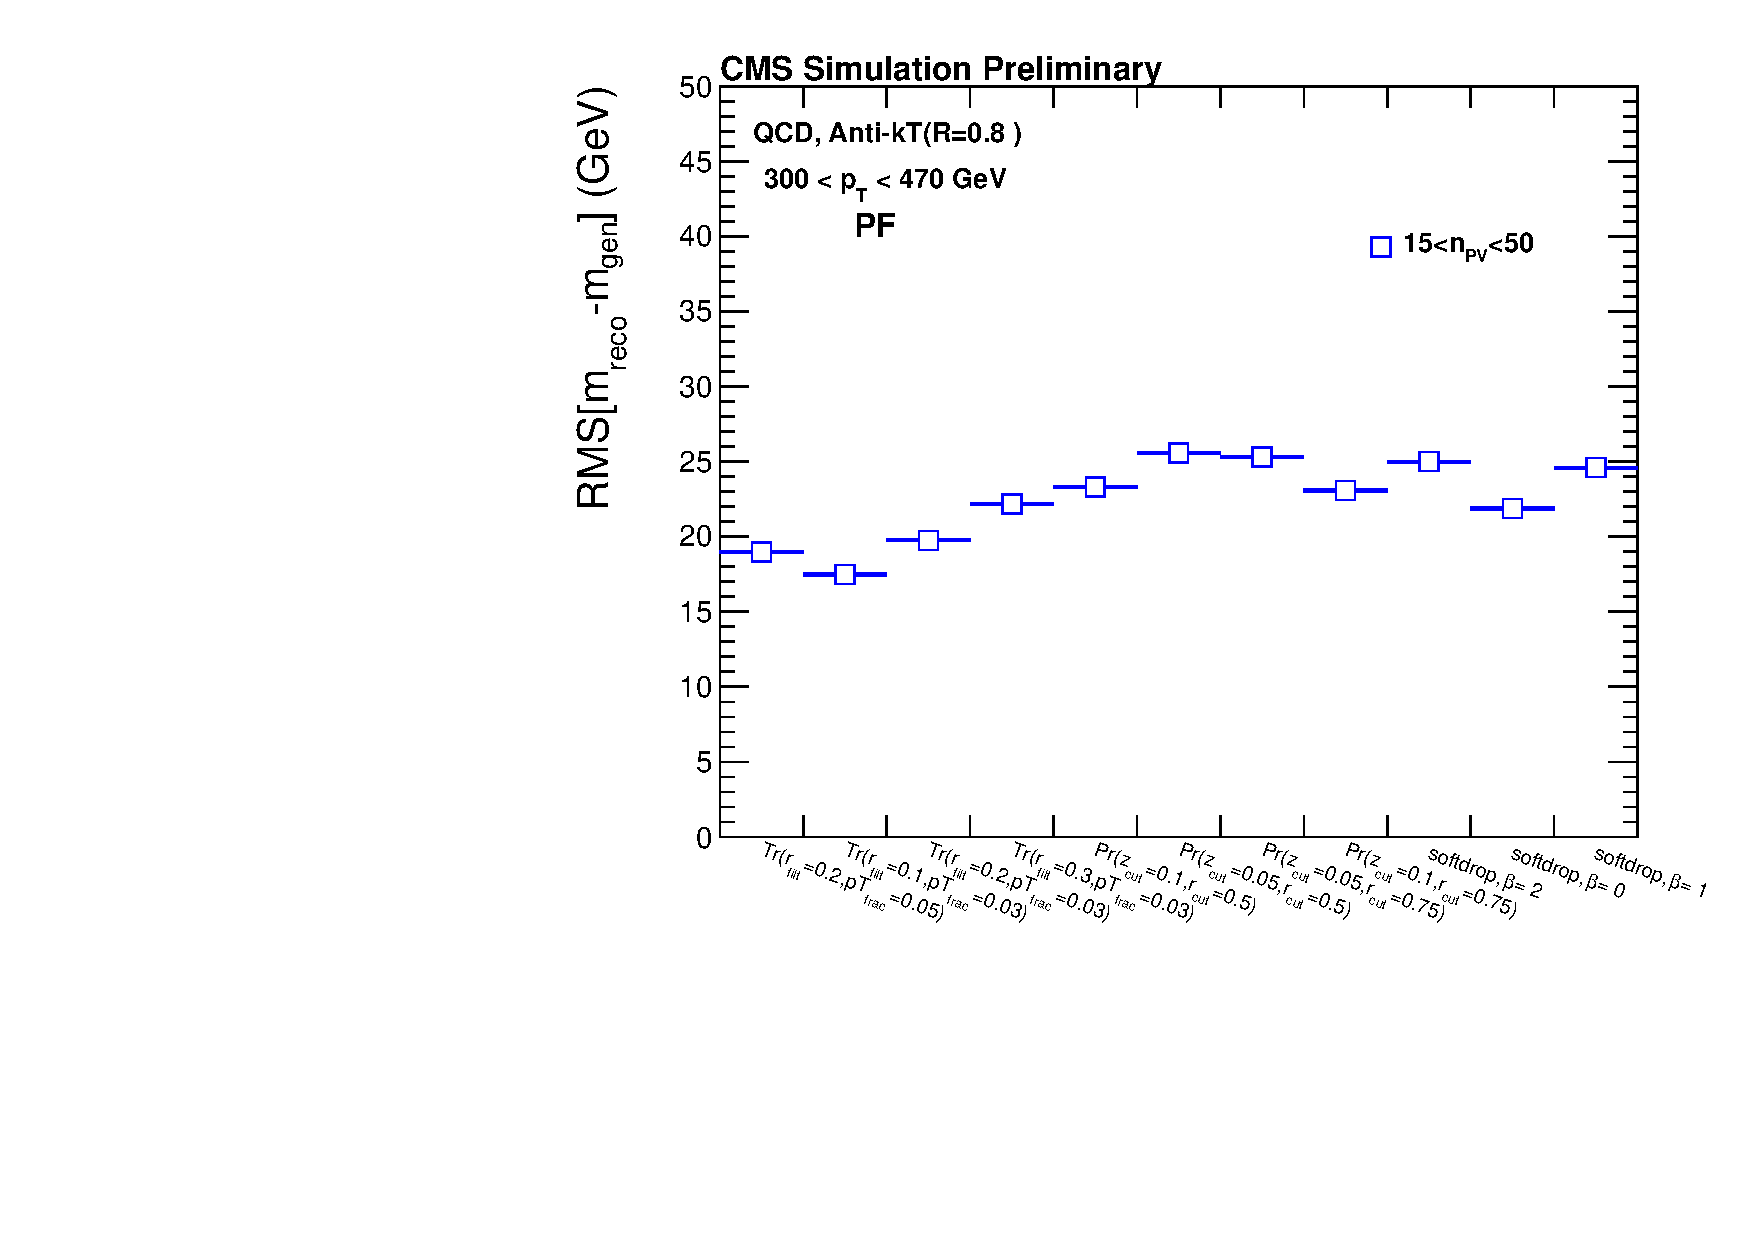
\includegraphics[width=0.47\textwidth]{/home/bibhu/Desktop/PhDThesis/PhDThesis/chapter8/SummaryPFallNPV.pdf}
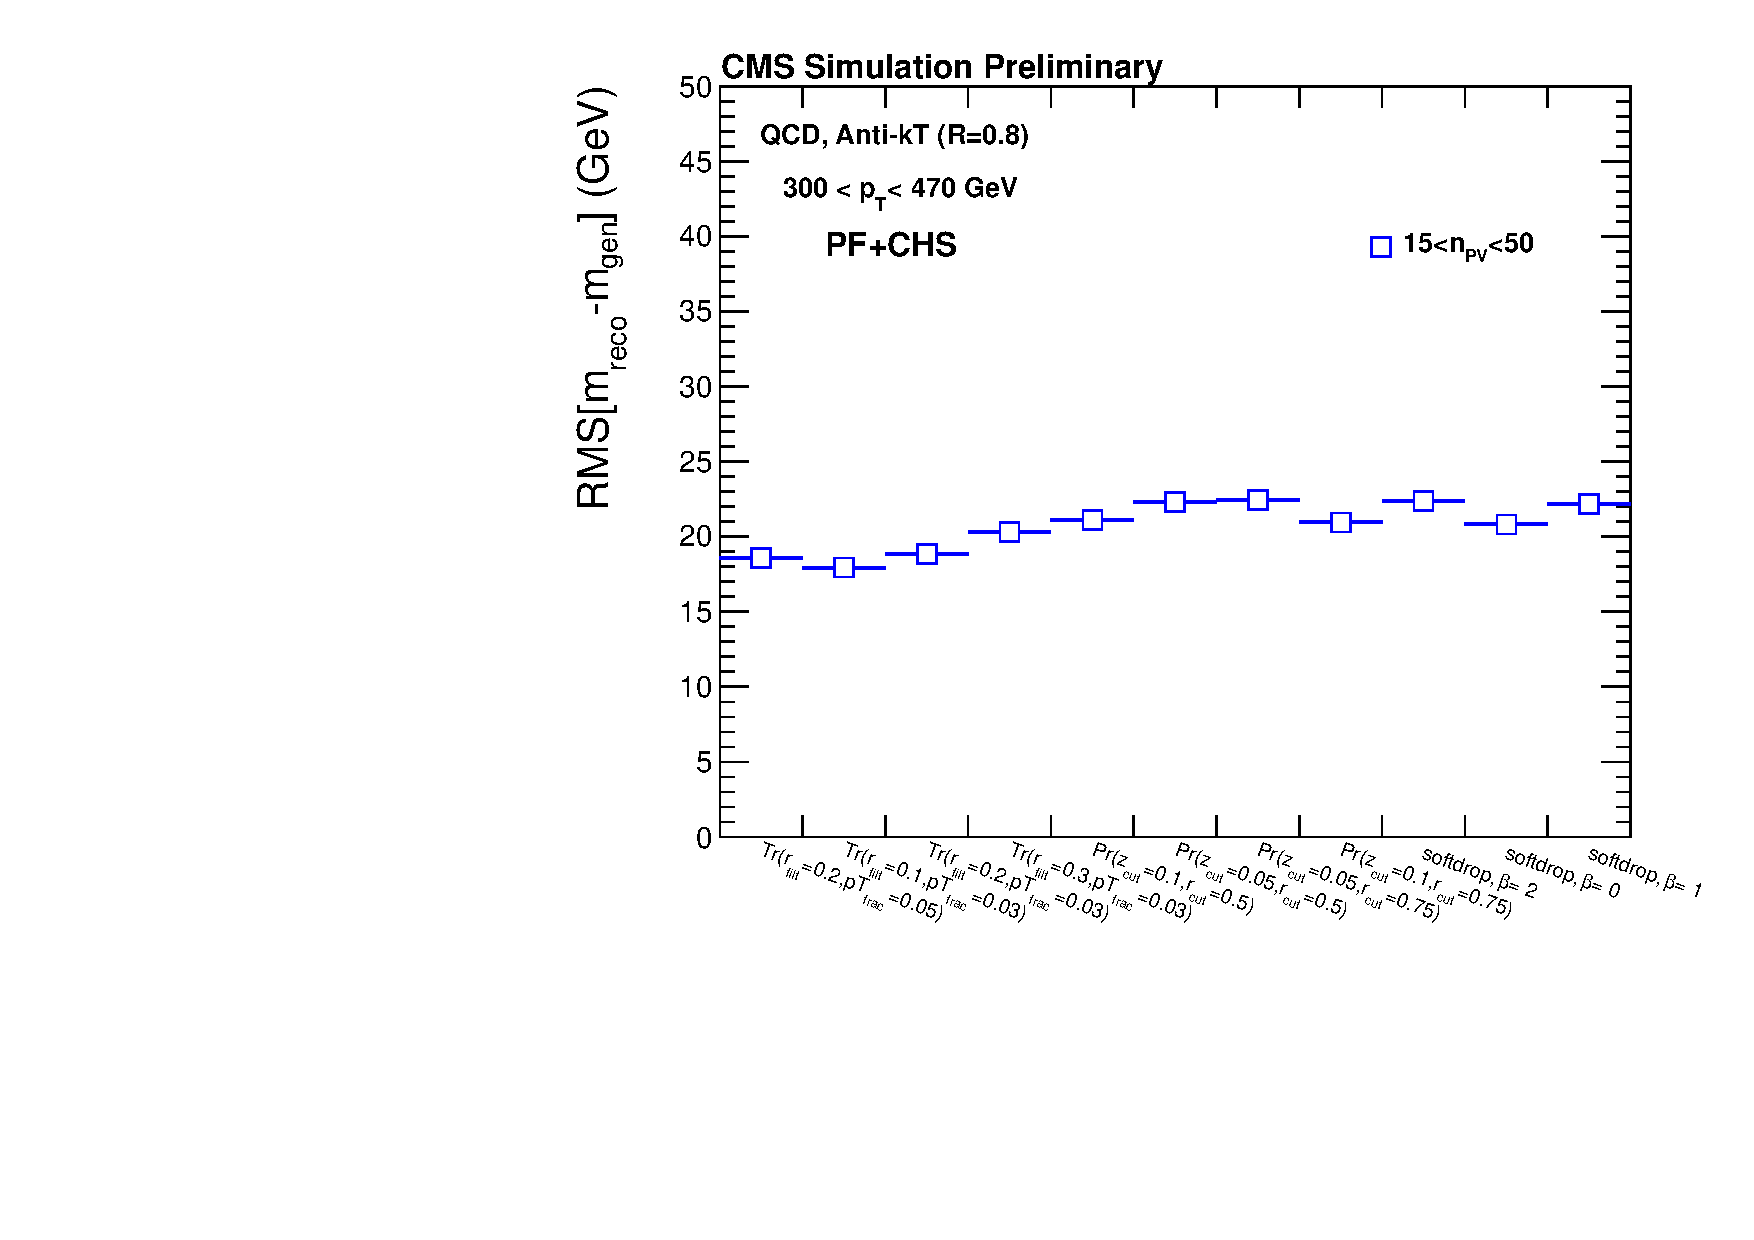
\includegraphics[width=0.47\textwidth]{/home/bibhu/Desktop/PhDThesis/PhDThesis/chapter8/SummaryPFCHSallNPV.pdf}\\
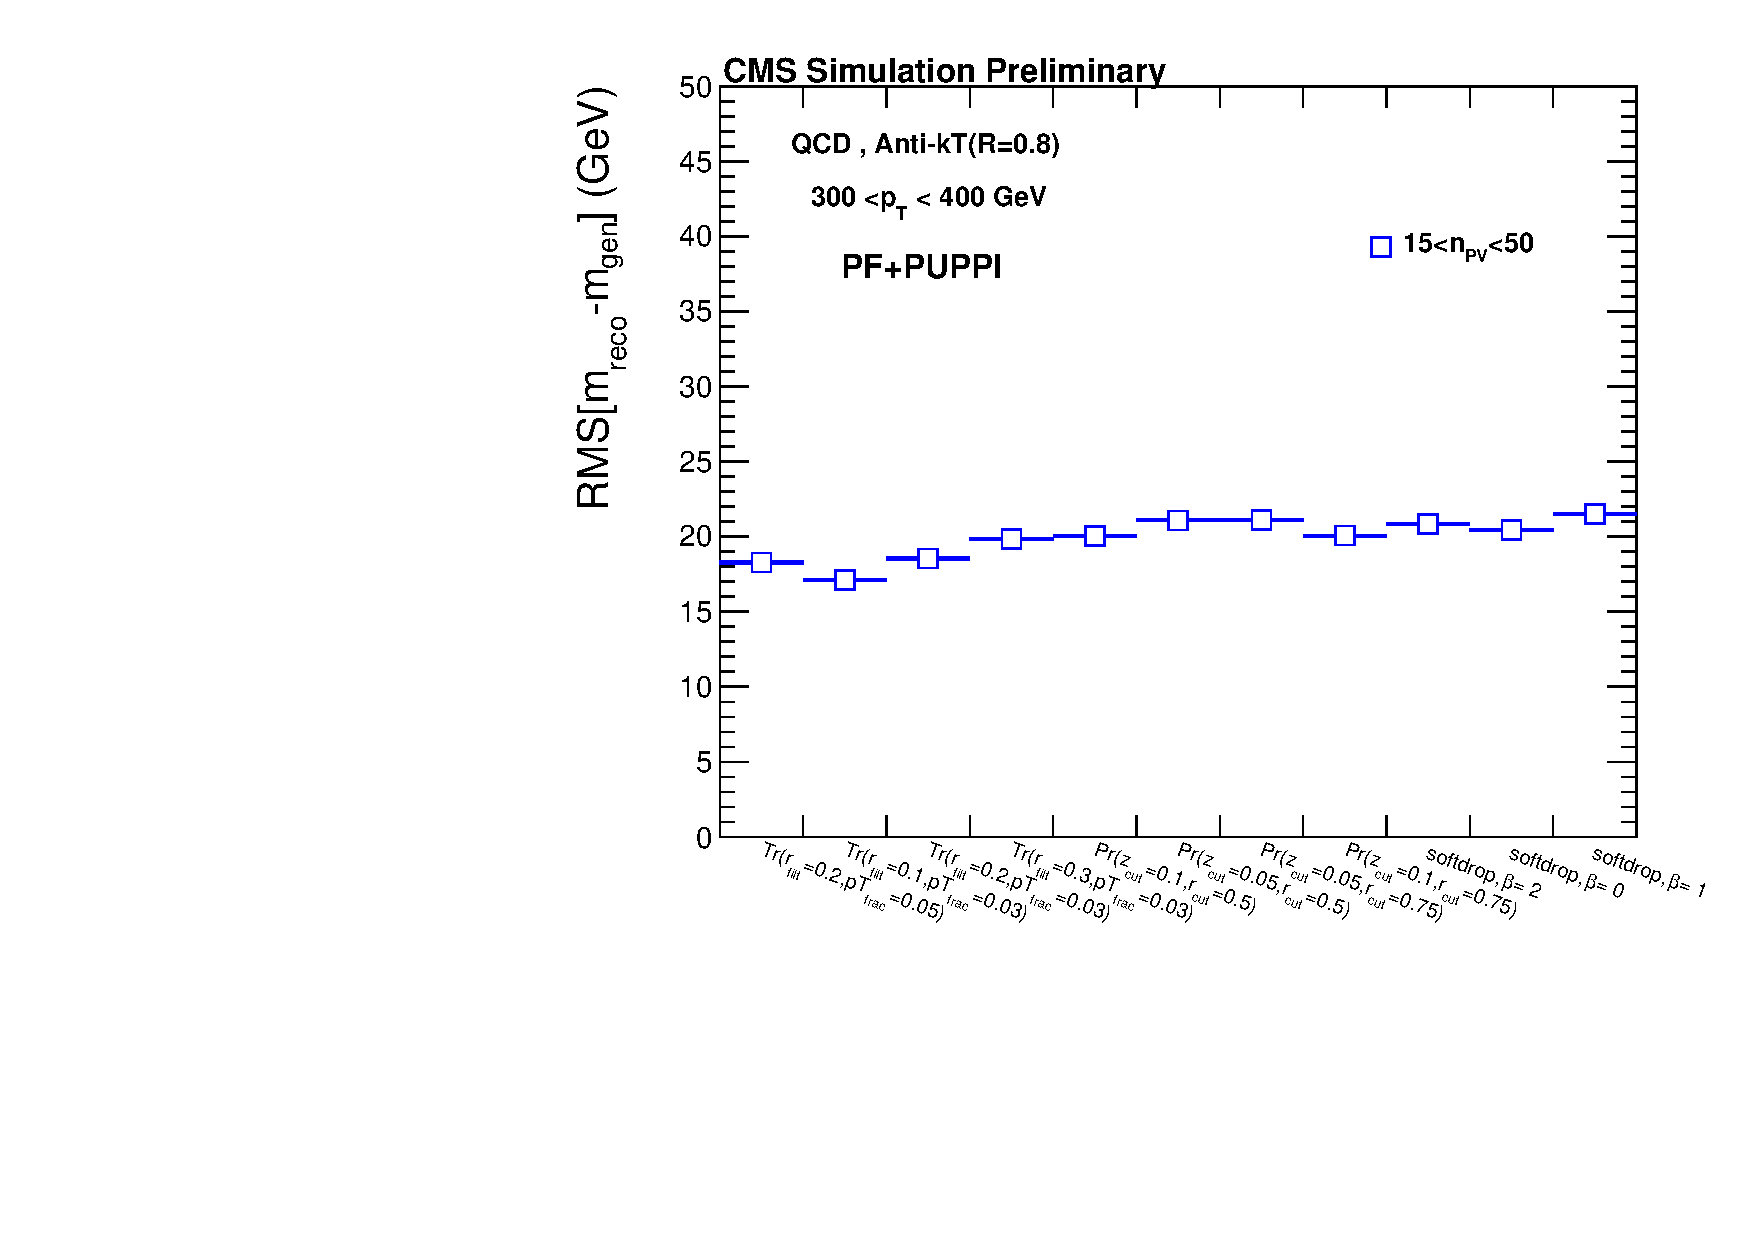
\includegraphics[width=0.47\textwidth]{/home/bibhu/Desktop/PhDThesis/PhDThesis/chapter8/SummaryPUPPIallNPV.pdf}
\caption{Comparison of jet mass resolution for PF, CHS and Puppi  with different grooming variables}
\label{fig:summary_all_groomer_QCD}
\end{figure}
















